\chapter{太阳能光热发电平台的试验研究}

第\ref{cha:Modeling}章介绍了利用MATLAB建模工具实现为太阳能光热发电系统中各关键部件建模的工作。基于其建立的部件模型,可以方便地构建太阳能光热发电平台的模型。

在第\ref{cha:Modeling}章中,建立了槽式集热器的机理模型。在假定整体传热系数沿着集热器长度方向均匀分布的条件下,建立了传热流体温升与太阳辐射强度、集热器长度、传热流体流量、环境温度、传热流体入口温度等因素之间的关系式,并得出了槽式集热器的热效率计算公式。
还详细分析了碟式接收器的各种能量损失,建立了详细的热网络模型。通过使用各种经典的传热公式,求解了热网络模型中各节点温度值,并得到了碟式集热器的热效率计算公式。

%For organic Rankine cycle (ORC) system, processes of the Rankine cycle were analyzed and the Rankine cycle efficiency formula is derived.
为了更加深入地理解太阳能光热发电系统,也为了对所提出的部件模型进行验证分析和误差分析,建立了包括太阳能槽式集热器、太阳能碟式集热器、有机工质朗肯循环系统(ORC系统)的太阳能光热发电平台。该平台的建立为以后太阳能梯级集热系统的搭建提供了良好的基础。

\section{平台简介}

\begin{figure}[!ht]
\centering
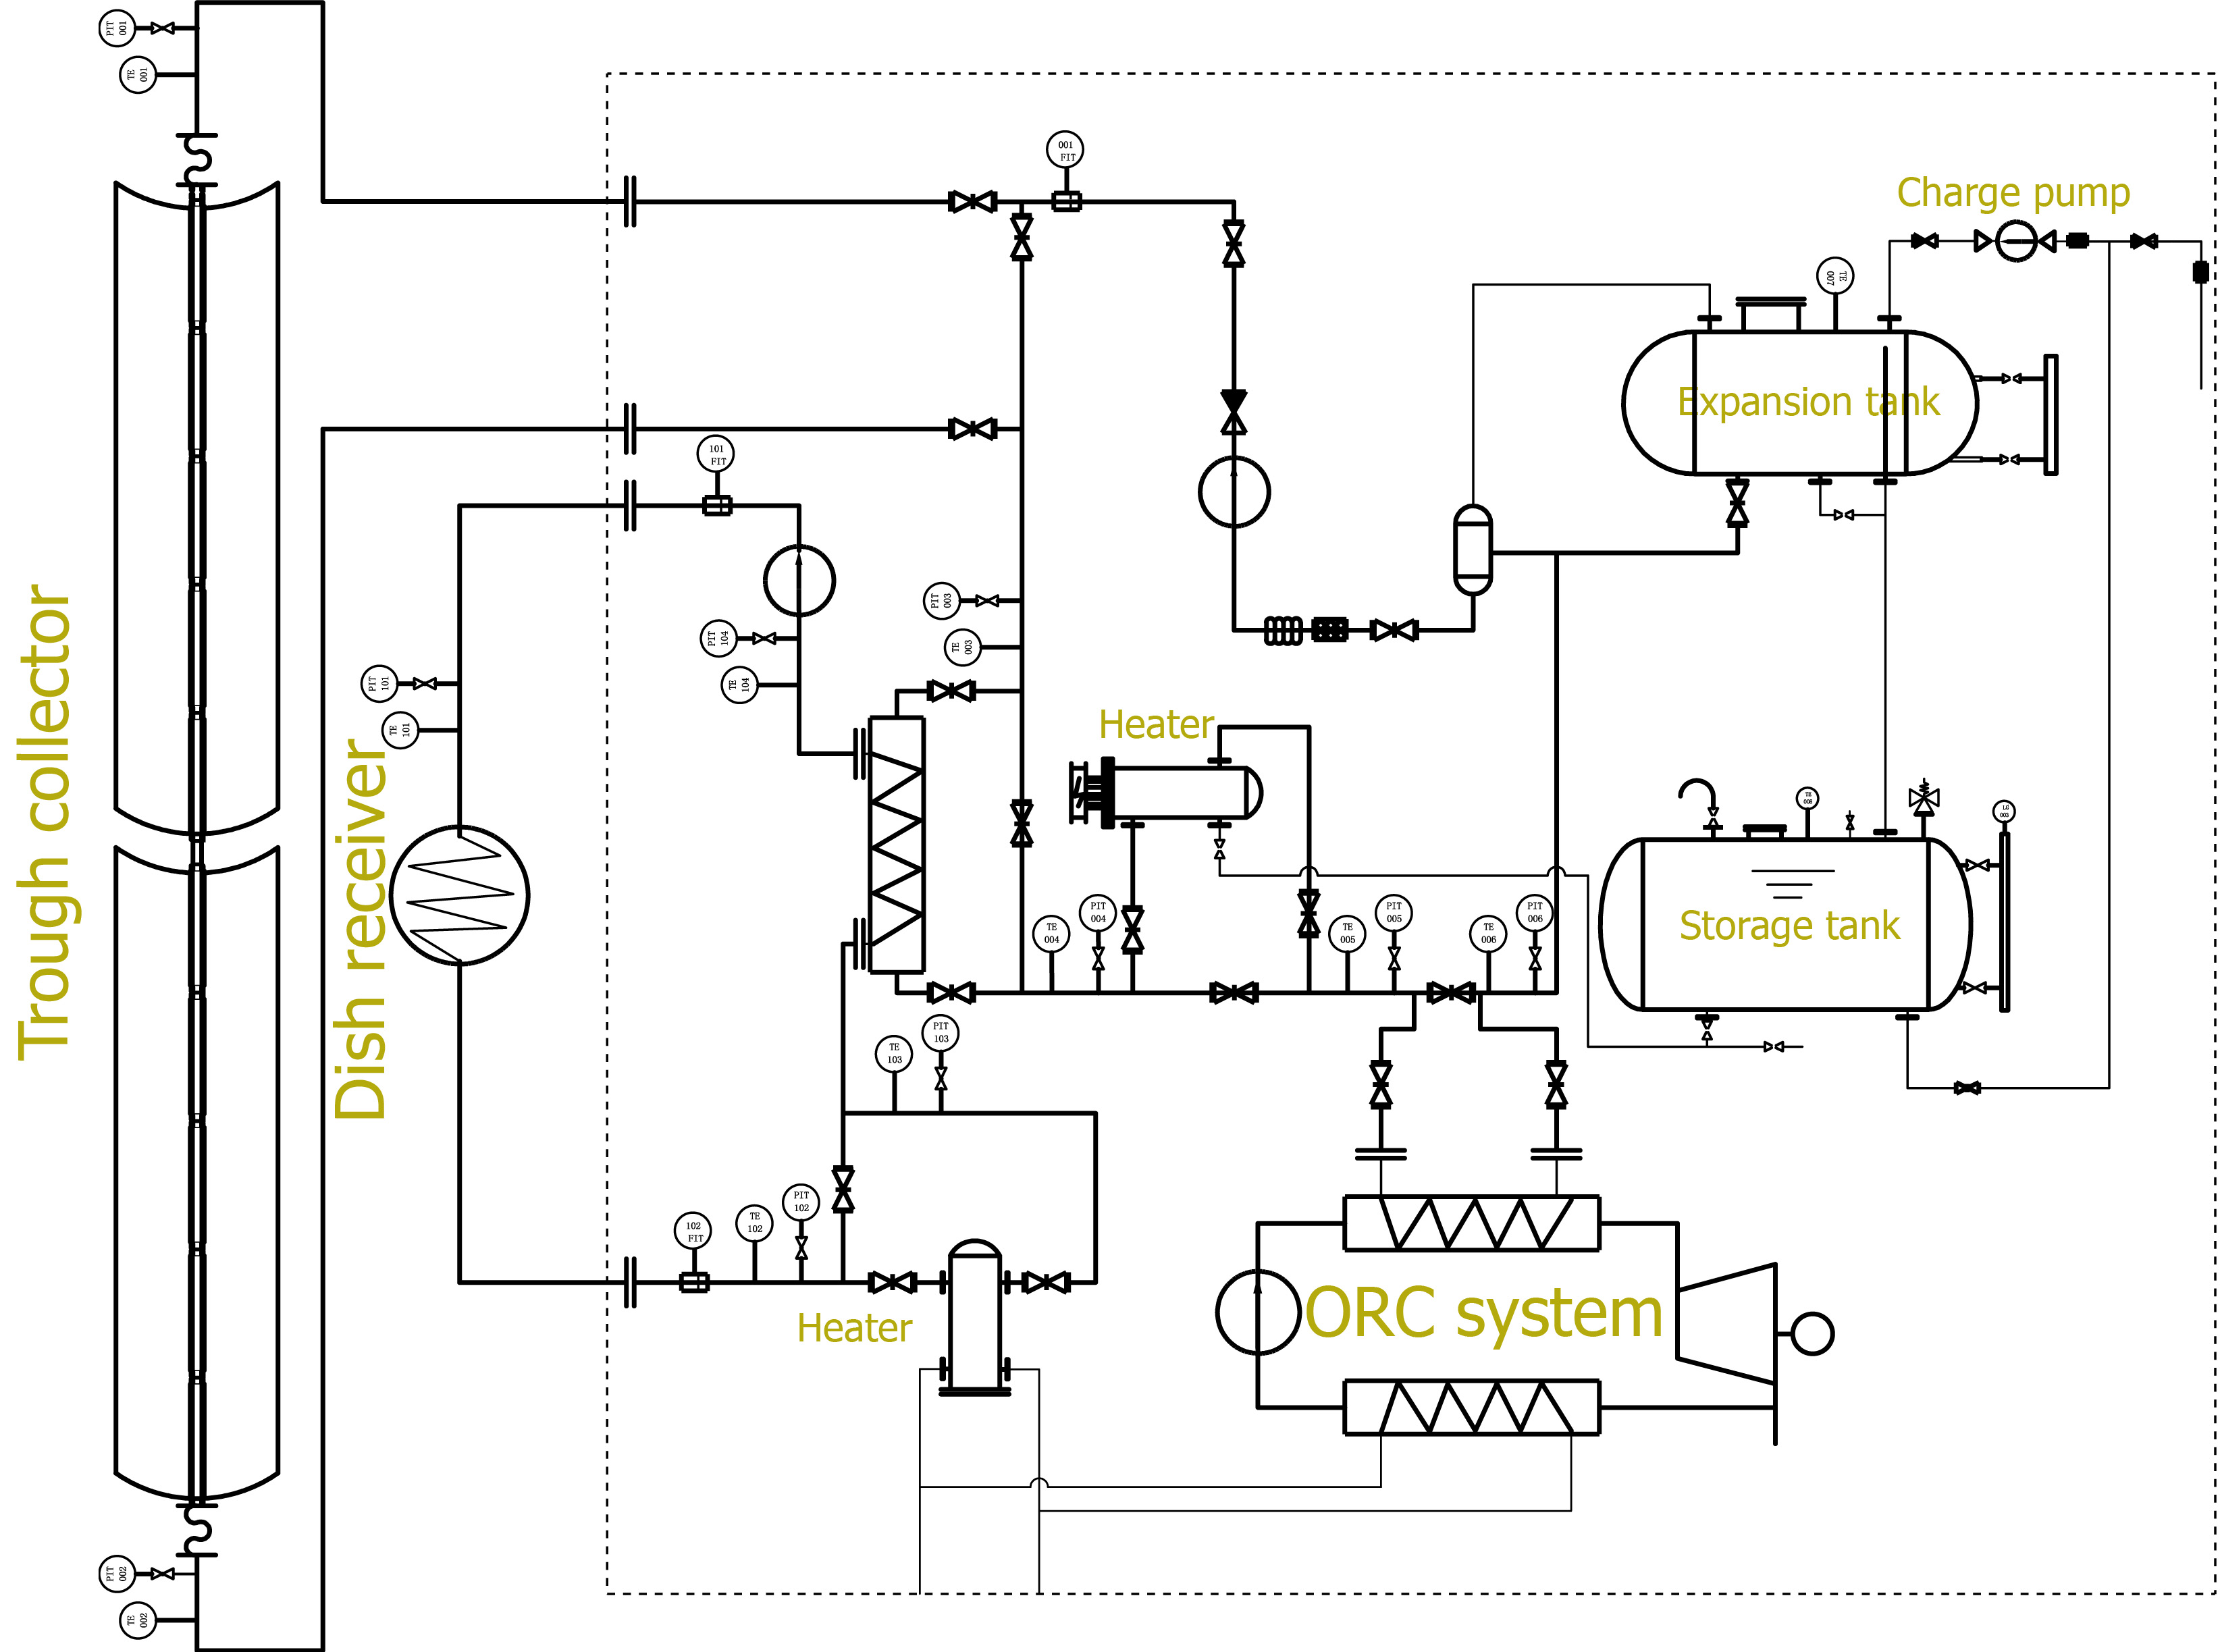
\includegraphics[width=1.0\textwidth]{fig/platform.jpg}
\caption{太阳能光热发电平台的结构示意图}\label{fig:platform}
\end{figure}
太阳能光热发电平台的结构示意图如图\ref{fig:platform}所示。不同的流体构建了三个回路,包括空气回路、油回路和有机工质回路。
在空气回路中,环境中的空气首先在空气压缩机中被加压,再送到碟式集热器中实现高温集热,经过空气-油换热器将获得的热量提供给朗肯循环,再经过冷却系统排至大气中。此外,空气回路还设有加热器支路,可以将空气预热之后再送入碟式集热器中,以便于研究不同空气入口温度对碟式集热器热效率的影响。
在油回路中,导热油先被槽式集热器加热,然后流入空气-油换热器吸收热空气提供的热量,接着流入ORC系统的蒸发器,为朗肯循环提供热量后再经油泵泵入槽式集热器。此外,油回路还设有加热器支路,可以将导热油再次加热之后再送入ORC系统,可以将导热油加热至指定温度,为ORC系统提供温度稳定的热源。
在有机工质回路中,有机工质流体在蒸发器中吸收热量,变成蒸气,进入有机工质汽轮机膨胀做功,接着流入回热器回收部分热能,然后通过有机工质泵回到蒸发器。

接下来将详细介绍太阳能光热发电平台的重要设备。

\subsection{碟式集热器}
由于土地限制,碟式集热器呈沿东西方向布置。它由槽式反射镜、接收器和支架组成,其结构如图\ref{fig:TroughCollector}所示。槽式反射镜长20$\,\mathrm{m}$,宽2.55$\,\mathrm{m}$。接收器采用的是北京桑普公司的SEIDO-I系列产品,它由黑色的金属吸热管和透明的玻璃管组成,二者之间抽成真空以减少散热损失。玻璃管的外径为0.11$\,\mathrm{m}$,内径为0.106$\,\mathrm{m}$,金属管的外径为0.038$\,\mathrm{m}$,内径为0.035$\,\mathrm{m}$。金属和玻璃采用溶封(火封)连接,玻璃管和金属管之间起始真空度保持在0.05 Pa左右,真空管内设有消气剂或其他保持真空的装置。支架用于支撑反射镜和接收器,其结构足以抵御市内的大风、雷电及雨雪等恶劣天气。槽式系统采用单轴跟踪系统,水平回转角度为-85$^\circ$至+175$^\circ$,能够实行太阳监测并运算太阳轨迹,跟踪误差小于0.2°,没有累计误差。此外,除了自动跟踪模式以外,跟踪系统还提供了手动模式,控制柜中的控制按钮可以方便地将集热器调整到指定方位。跟踪系统还提供了在发生意外事故的条件下系统自动切换至自动保护的功能。
整个槽式集热器系统装置的转动、定位和连接等机械结构简单可靠,便于安装、拆装和运输,运行和维护方便;能够连续24小时稳定工作。

槽式集热器选用长城润滑油L-QD350合成型导热油作为传热介质,其典型参数由商家提供。

\begin{figure}[!ht]
\centering
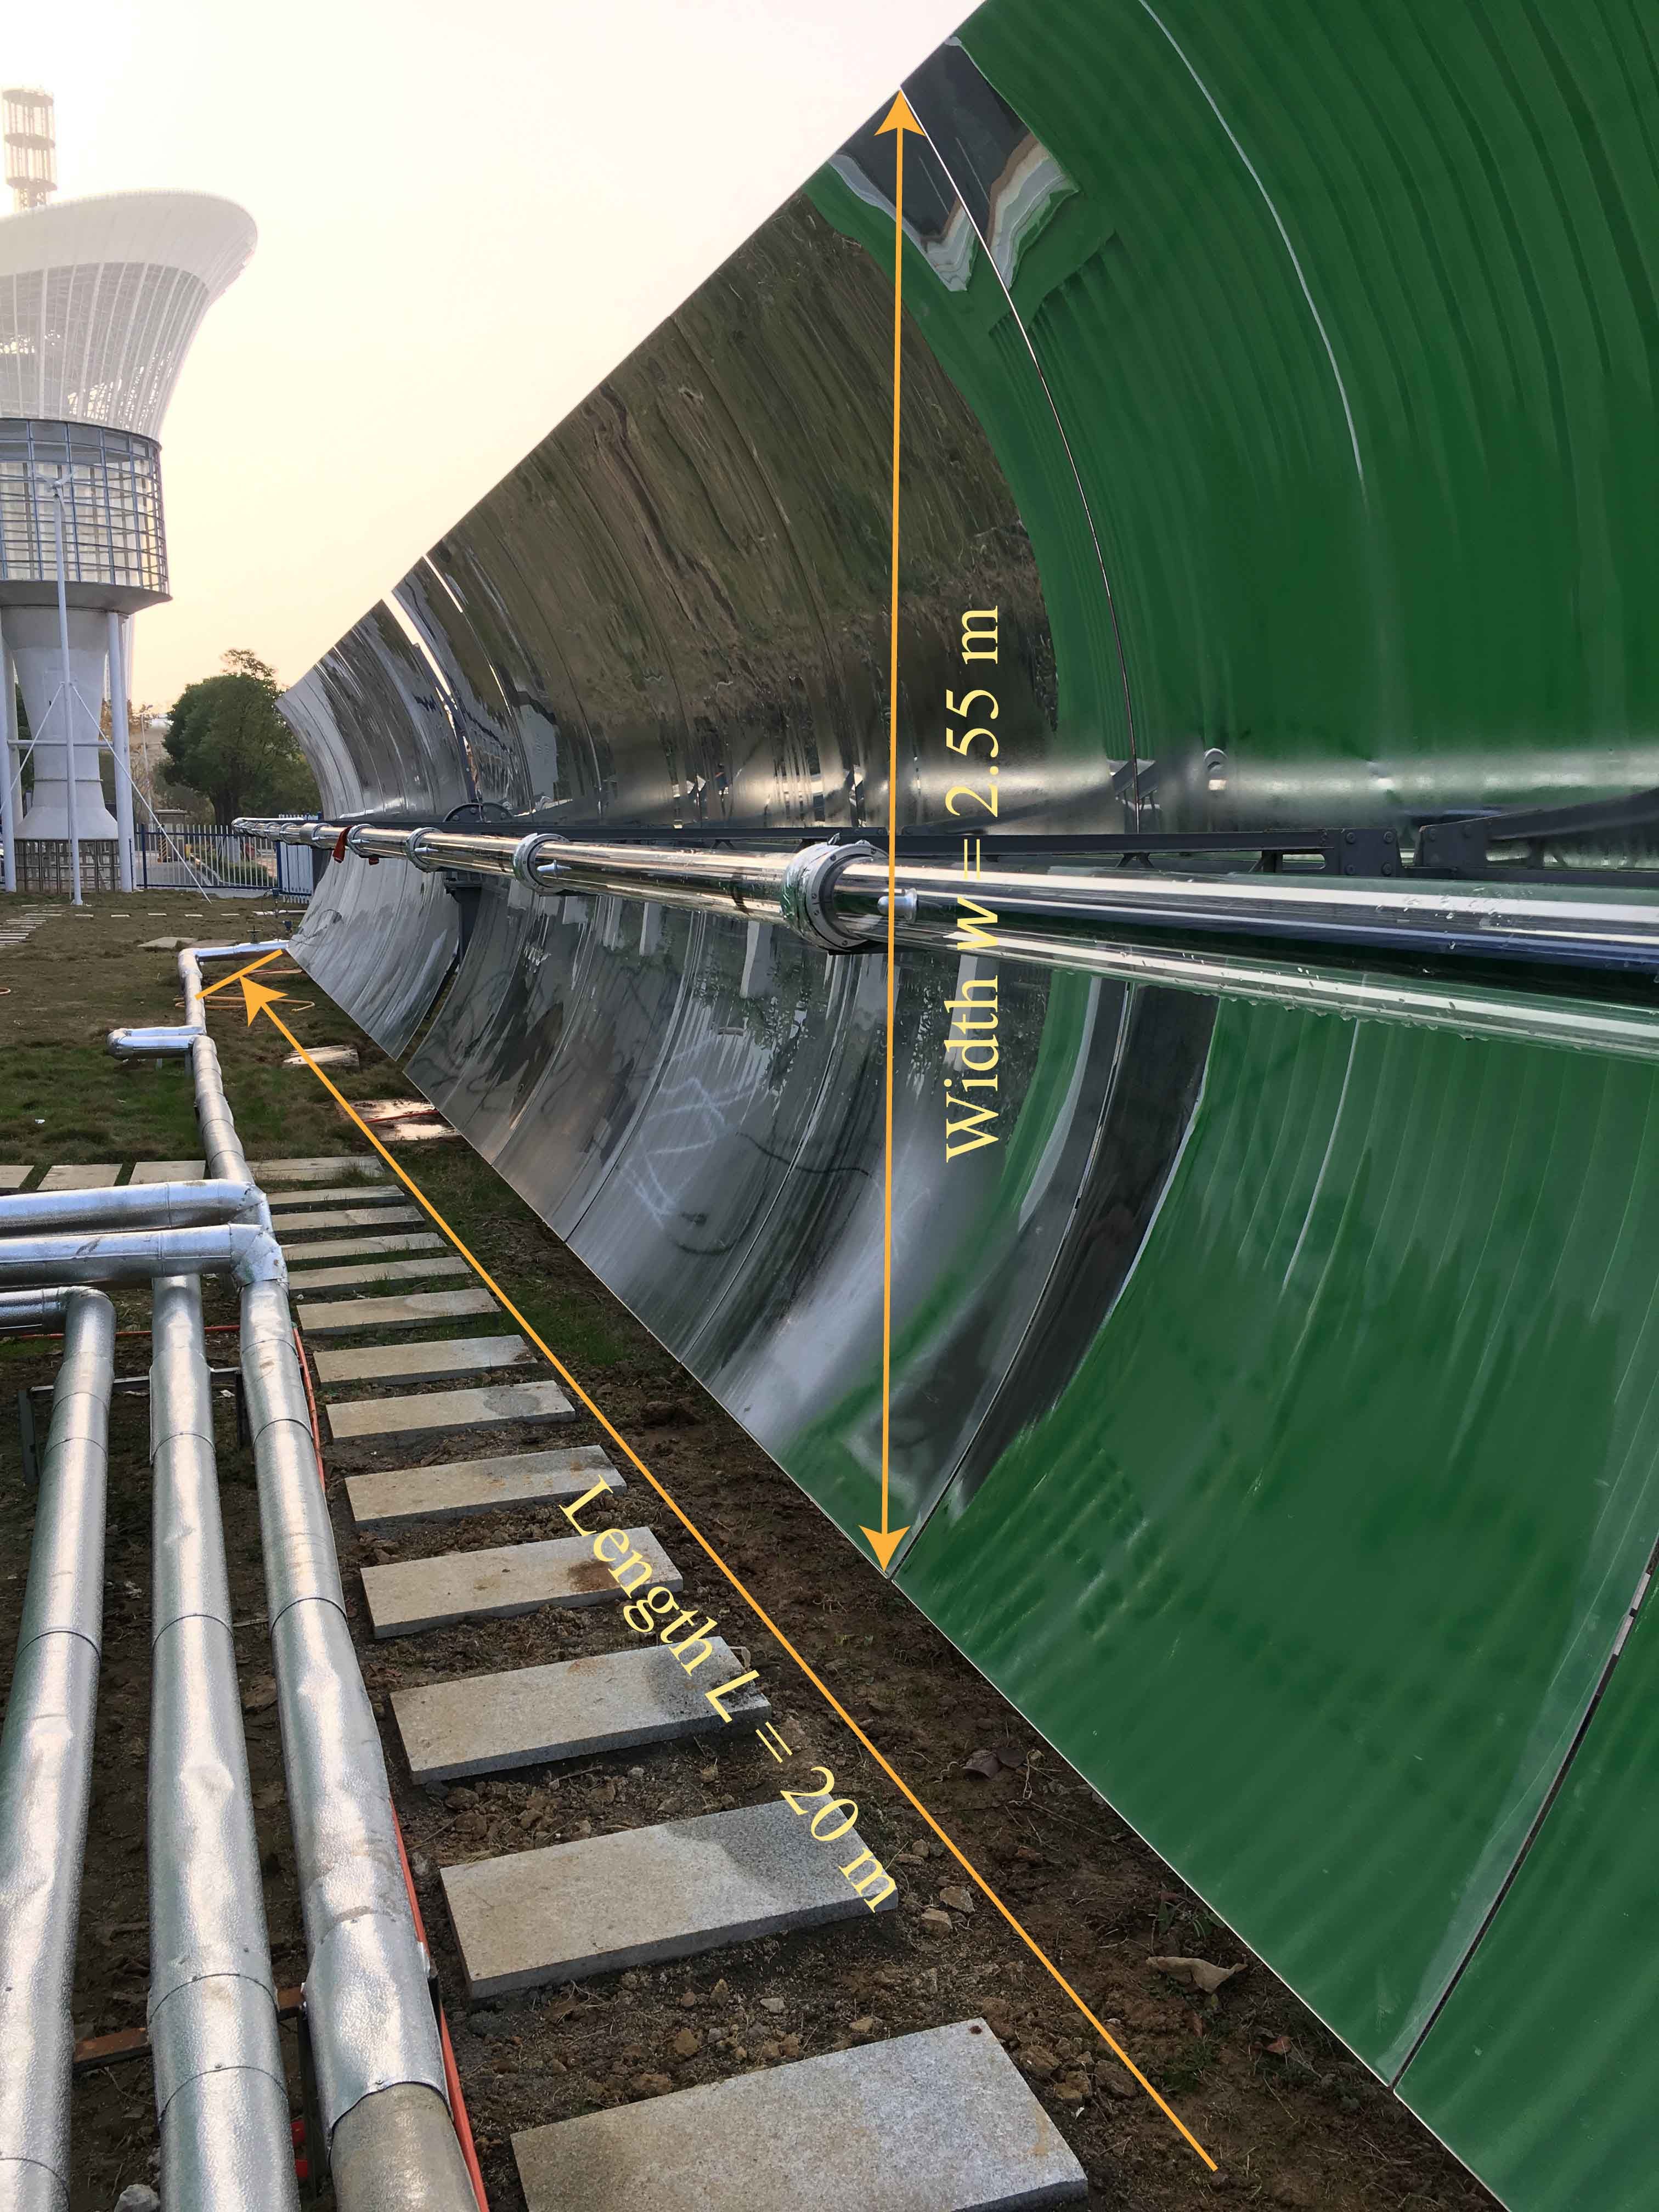
\includegraphics[width=0.7\textwidth]{fig/TroughCollector.jpg}
\caption{试验平台的槽式集热器}
\label{fig:TroughCollector}
\end{figure}

\subsection{碟式集热器}

\begin{figure}[!ht]
\centering
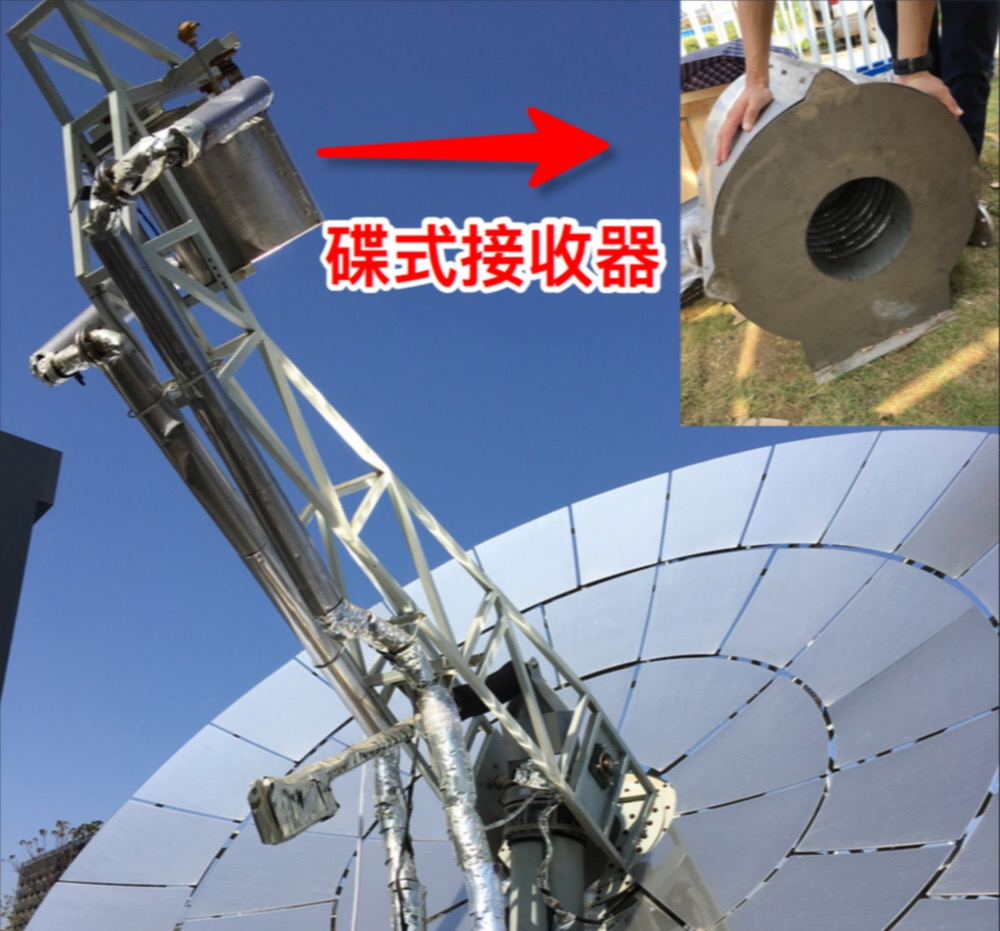
\includegraphics[width=0.7\textwidth]{fig/DishCollector.jpg}
\caption{试验平台的碟式集热器}
\label{fig:DishCollector}
\end{figure}
碟式集热器的实物图如图\ref{fig:DishCollector}所示,其镜面由多块弯曲成型的玻璃反射面组成。当集热器开口正对太阳时,每块玻璃反射面都将入射光线反射到集热器的焦点处。
集热器的焦点放置有自行设计的接收器,如图\ref{fig:DishCollector}的顶部所示。
碟式集热器的各重要参数见表\ref{tab:ddc}。
\begin{table}[htbp]
	\caption{碟式集热器的重要参数列表}
	\begin{center}
	\begin{tabular}{cccccc}
		\toprule
		参数		&	值	&	参数		&	值	&	参数		&	值\\
		\midrule
		$d_{cav}$	&	0.45$\,\mathrm{m}$	&	$\epsilon_{insu}$	&	0.6	&	$\theta_{dc}$	&	20$^\circ$\\
		$\delta_{insu}$	&	0.11$\,\mathrm{m}$	&	$\alpha_{cav}$	&	0.87	&	$\gamma$	&	0.97\\
		$dep_{cav}$	&	0.45$\,\mathrm{m}$	&	$\delta_a$		&	0.002$\,\mathrm{m}$	&	$\eta_{shading}$	&	1\\
		$d_{ap}$	&	0.25$\,\mathrm{m}$	&	$d_{i,1}$	&	0.07$\,\mathrm{m}$	&	$\rho$	&	0.91\\
		$\lambda_{insu}$	&	0.06$\,\mathrm{W/(m\cdot K)}$	&	$A_{dc}$	&	23.3$\,\mathrm{m^2}$	&	\\		
		\bottomrule
	\end{tabular}
	\end{center}
	\label{tab:ddc}
\end{table}
碟式集热器采用YYGN-GR-1A型双轴跟踪系统,该跟踪系统同时采用算法跟踪和传感器跟踪。同样,除了自动跟踪功能外,该跟踪系统也提供了手动调整集热器朝向的功能。通常在进行聚焦工作时,先启用手动模式,将集热器粗略调整至朝向太阳的方向,然后再启用自动模式,利用传感器精确对准太阳,并启用跟踪算法,实现连续精确地跟踪太阳。这为碟式集热器提供了非常精确的跟踪方式,其误差小于0.2$^\circ$,且没有累积误差。

碟式集热器的控制柜提供了机械电气等控制功能。它还提供了对环境风速的实时监测结果,可以设定极限风速。当环境风速达到设定的极限风速时,系统将启用保护动作,将碟式集热器旋转至安全角度(朝向天顶)。

\subsection{有机工质朗肯循环系统}
ORC系统选用的是法国公司Enogia的产品,整个ORC系统放置在长1.2米,宽0.8米,高1.7米的钢架结构中,其系统结构示意图和实物图分别如图\ref{fig:ORCsystemScheme}和图\ref{fig:ORCsystem}所示,ORC系统由汽轮机、发电机、回热器、凝汽器、缓冲罐、泵、蒸发器、控制柜、润滑冷却系统等部件组成。
\begin{figure}[!ht]
\centering
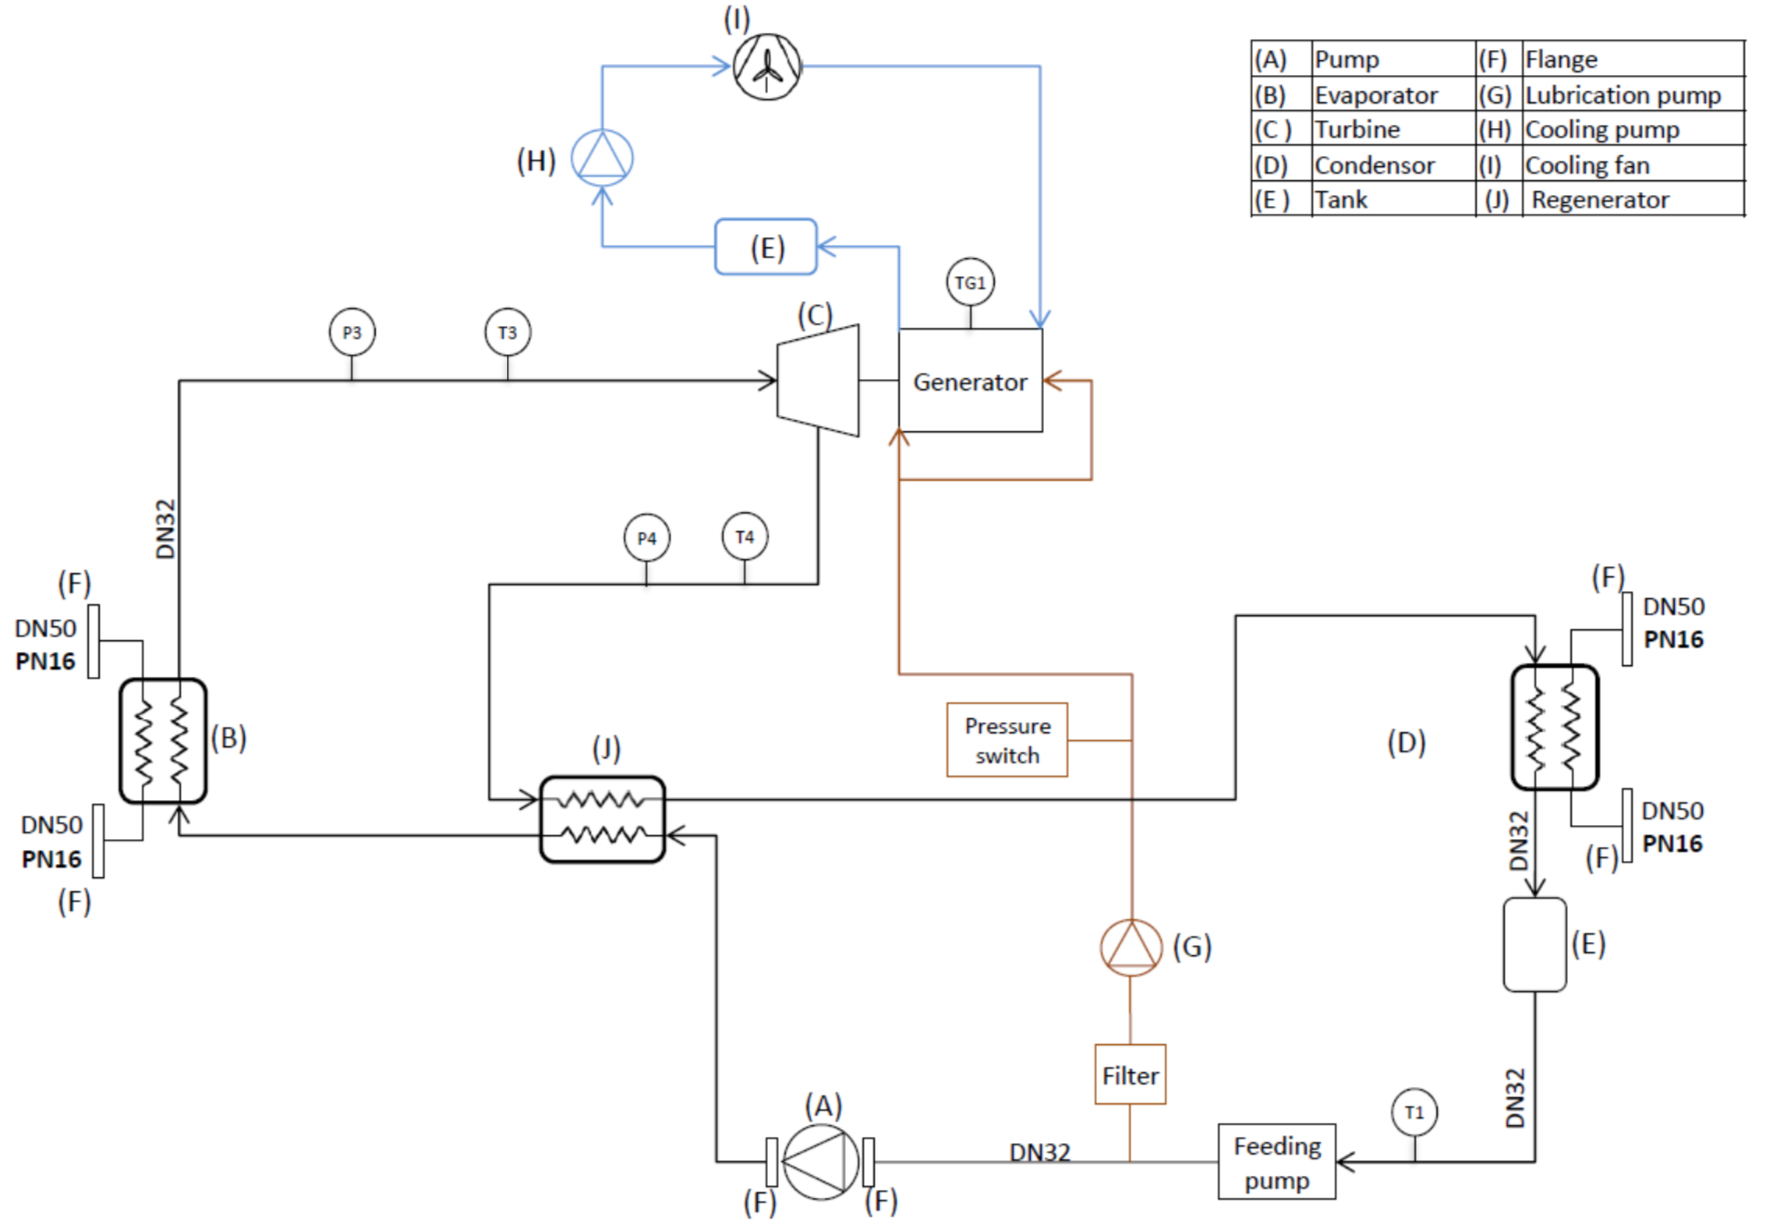
\includegraphics[width=0.7\textwidth]{fig/ORCsystemScheme.jpg}
\caption{ORC系统结构示意图}
\label{fig:ORCsystemScheme}
\end{figure}
\begin{figure}[!ht]
\centering
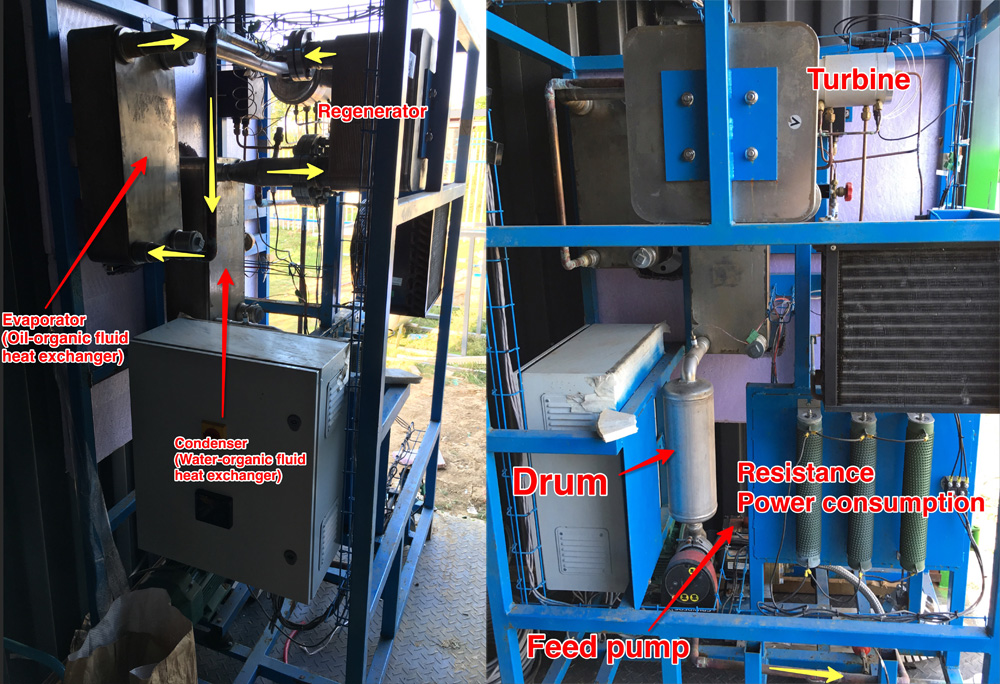
\includegraphics[width=0.7\textwidth]{fig/ORCsystem.jpg}
\caption{ORC系统实物图}
\label{fig:ORCsystem}
\end{figure}

ORC系统采用导热油作为热源,采用自来水作为冷源。在热回路中,额定工况下,导热油的入口温度为180$\mathrm{^\circ C}$,出口温度为160$\mathrm{^\circ C}$,质量流量为0.44$\,\mathrm{kg/s}$。在冷回路中,额定工况下,冷却水的入口温度为30$\mathrm{^\circ C}$,质量流量为0.83$\,\mathrm{kg/s}$。额定工况的输出功率为1.5$\,\mathrm{kW}$。

控制柜提供了触摸屏来控制ORC系统,控制柜提供了自动运行模式和手动操作模式。在自动运行模式下,所有的启动工作和关停工作都由程序设定自行完成,系统根据当前热源和冷源的情况自行调整输出功率。在手动模式下,可以手动调节系统运行参数,如有机工质泵的频率,来对系统进行精确调节。

\begin{figure}[!ht]
\centering
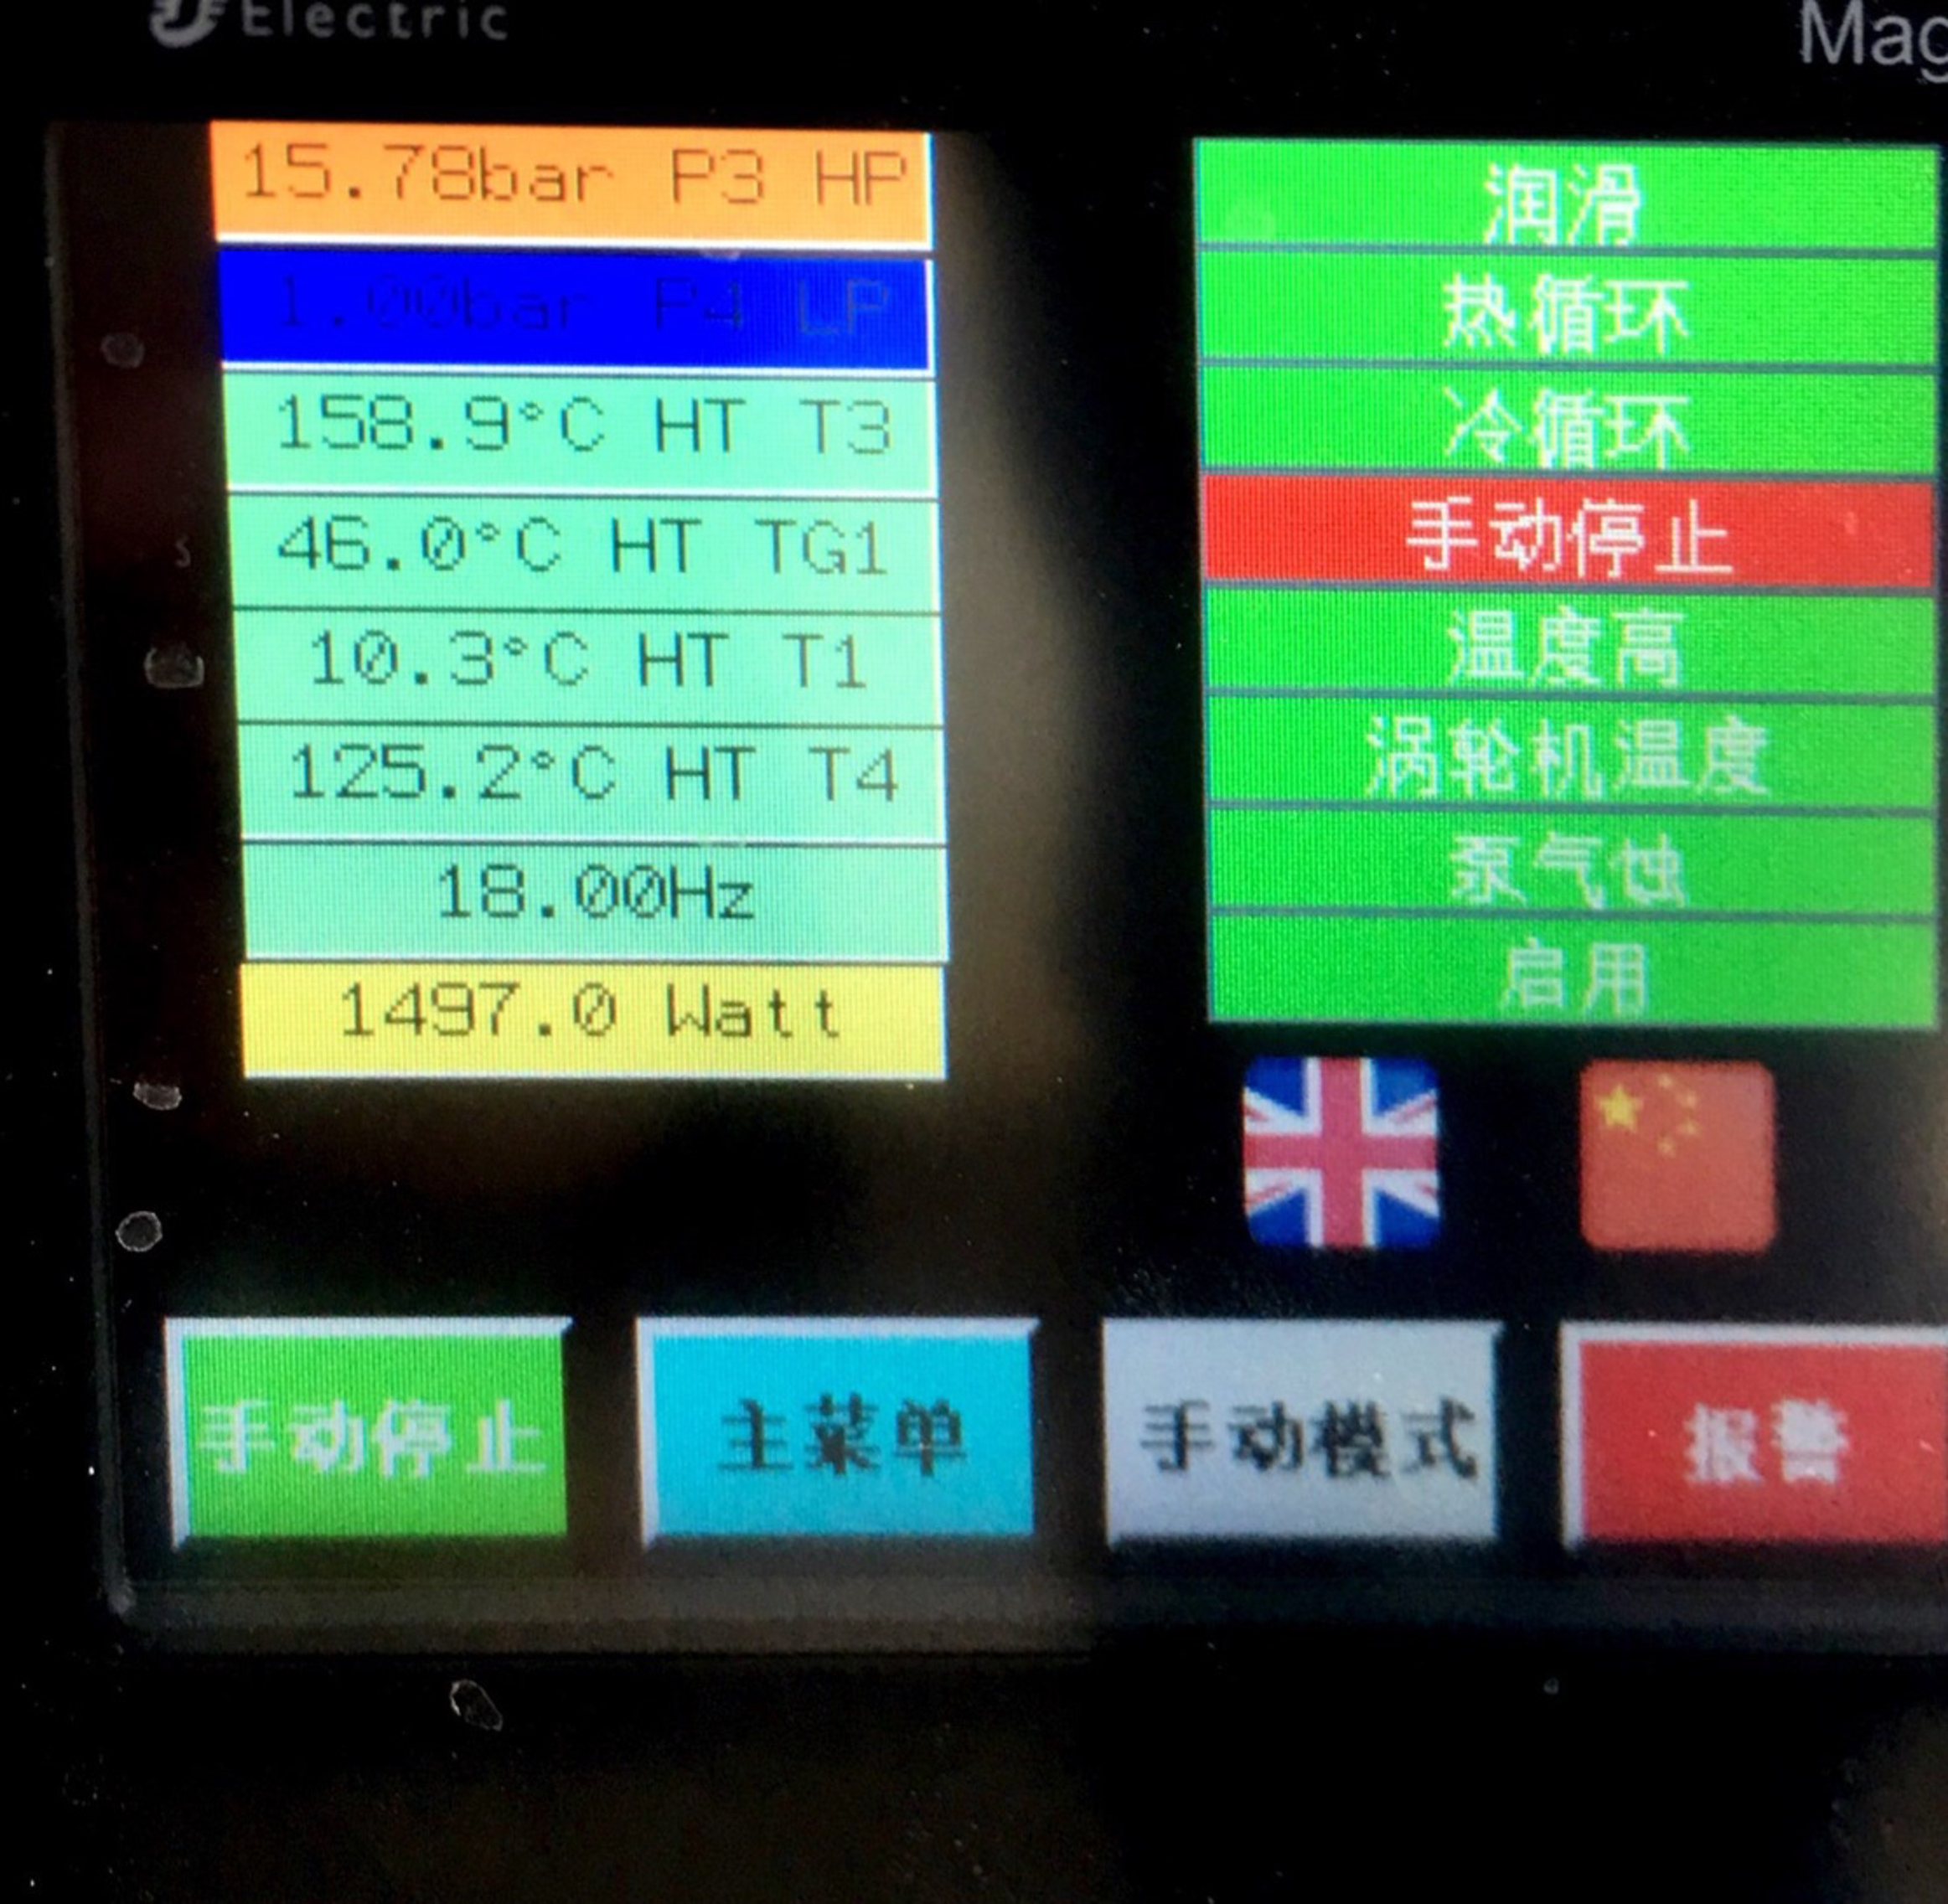
\includegraphics[width=0.4\textwidth]{fig/ControlCabinet}
\caption{ORC系统控制柜的操作界面}\label{fig:ControlCabinet}
\end{figure}

需要指出的是,由于ORC系统在运输和存放过程中,汽轮机末端轴承产生了损伤。ORC系统不能连续稳定运行,需要待法国工程师更换轴承后再进行相关试验工作。此外,由于本文所采用的有机工质朗肯循环模型是经典模型,ORC系统的效率计算公式同样采用该模型。所以,本文所采用的有机工质朗肯循环模型无需也不能采用ORC试验的数据进行验证。

\subsection{管道系统}

管道系统提供了流体流动和换热的基础。此外,它还铺设了保温层以减少热流体的对环境的散热。管道中布置了测量仪表、泵、阀门、罐体及加热器等器件来维持系统正常有序地运行。

太阳能光热发电平台采用了两个加热器来调节流体(空气和导热油)的温度,以满足试验的要求。
两个加热器都可以通过改变功率来维持其出口流体温度的稳定。
此外,当太阳辐射强度不够高时,可以启用加热器辅助加热,实现ORC系统的正常运行。
%\subsection{Data collection system}

\section{试验}

为了测试平台的性能并验证本文建立的部件模型,进行了相关的试验操作。

\subsection{槽式集热器试验}
\subsubsection{试验目的}
槽式集热器试验的目的是研究太阳辐射强度、传热流体流量、入口温度对槽式集热器热性能的影响,并验证第\ref{sec:ptc}节所建立的槽式集热器模型。

\subsubsection{试验步骤}
试验步骤分为以下几步:
\begin{enumerate}[label=(\arabic*)]
	\item 完成准备工作。确保所有部件和仪表都正确连接,并可以正常工作。
	\item 初始化太阳能辐射仪。调整太阳能辐射仪的方向来获取太阳直射强度的数值,确保穿过辐射仪孔道的阳光落在校准位置。
	\item 打开油回路的阀门,并开启油泵。
	\item 打开槽式集热器跟踪系统的马达。同步跟踪系统的时间,并开启自动模式,让槽式系统自动对向太阳,并开始跟踪。
	\item 调整槽式系统参数来满足设计工况要求。当试验数据稳定后,记录并保存数据收集系统采集到的试验数据。
	\item 当所有设计工况测试完毕后,结束试验。
	\item 复位槽式集热器。在系统控制界面将槽式集热器调整至其开口水平的状态,关闭马达。
	\item 关闭油泵。
\end{enumerate}

\subsubsection{试验设计工况}

考虑到太阳直射辐射强度在晴天具有不可控性和相对连续性,当以太阳直射辐射强度为控制变量时,太阳辐射强度值不能控制为设计值,而应该为实测值。当需要固定太阳直射辐射强度时,应该尽量控制几组试验的总时间,以减少太阳直射辐射强度变化带来的影响。

\begin{table}[htbp]\footnotesize
	\caption{太阳能槽式系统的设计工况}
	\begin{center}
	\begin{tabular}{cccc}
		\toprule
		工况	& DNI($\mathrm{W/m^2}$)&	流量($\mathrm{kg/s}$)			&	入口油温($\mathrm{K}$)\\
		\midrule
		1-10	&	实测值	&	0.2	&	433.2\\
		11	&	实测值	&	0.1	&	433.2\\
		12	&	实测值	&	0.2	&	433.2\\
		13	&	实测值	&	0.3	&	433.2\\
		14	&	实测值	&	0.4	&	433.2\\
		15	&	实测值	&	0.5	&	433.2\\
		16	&	实测值	&	0.2	&	413.2\\
		17	&	实测值	&	0.2	&	423.2\\
		18	&	实测值	&	0.2	&	433.2\\
		19	&	实测值	&	0.2	&	443.2\\
		20	&	实测值	&	0.2	&	453.2\\
		\bottomrule
	\end{tabular}
	\end{center}
	\label{tab:DesignedCasesForTrough}
\end{table}

表\ref{tab:DesignedCasesForTrough}中,工况1到工况10分别在一天的不同时间点或是数天间的时间点完成。工况11到工况15的试验要求在半个小时之内完成。需要指出的是,当以入口油温为考察变量时,仅仅设计了5个温度相差不大的工况(工况16到工况20)进行试验。这是由于通过加热器提升油温的速度较慢,为了保证太阳辐射强度基本不变,所以各工况入口油温差别不大。这5个工况的试验要求在一个小时之内完成。

\subsubsection{数据处理方法}
%Outlet temperature of the oil in the trough collector is monitored and recorded. 
商家给定的导热油的比热容的数据为:当$T = 373.15\mathrm{^\circ C}$时,$c_p = 2.44\times10^3\,\mathrm{J/(kg\cdot K)}$;当$T = 473.15\mathrm{^\circ C}$时,$c_p = 2.88\times10^3\,\mathrm{J/(kg\cdot K)}$。本文假定导热油的比热容与温度成线性关系,采用线性插值法,则有$c_p = aT + b$,其中$a = 4.4\,\mathrm{J/(kg \cdot K^2)}$,$b = 798.14\,\mathrm{J/(kg\cdot K)}$。

导热油吸收的热量 $Q_{abs} = \int_{T=T_i}^{T = T_o}c_p\dot{m}dT = \dfrac{1}{2}a(T_o^2 - T_i^2)\dot{m} + b (T_o - T_i)\dot{m}$.

槽式集热器的集热效率
\begin{equation}
	\eta_{tc} = \dfrac{Q_{abs}}{I_rw_{tc}L_{tc}}
	\label{eq:ExperimentEta}
\end{equation}

为了验证本文建立的槽式集热器的模型的正确性,需要检查方程(\ref{eq:CTCHF})。在模型中,

\begin{equation}
	\widetilde{T_{o}}=T_{amb} + \dfrac{q''}{U(T_{abs})} + \exp(-\frac{U(T_{abs})\pi d_o L}{\dot{m}\widetilde{c_p}})(T_{i}-T_{amb}-\dfrac{q''}{U(T_{abs})})
	\label{eq:CheckT_o}
\end{equation}

其中,$T_{abs}$用$(T_i + T_o)/2$代替($T_i$和$T_o$分别采用测量的入口油温和出口油温),$\widetilde{c_p}$是用$(T_i + T_o)/2$得到的平均比热容。
$U(T_{abs})$由下式得到\cite{Romero2007}:
\begin{equation}
	U(T_{abs}) = 0.687257 + 0.001941(T_{abs} - T_{amb}) + 0.000026(T_{abs} - T_{amb})^2
	\label{eq:U_T_abs}
\end{equation}
\begin{equation}
	q'' = \frac{I_r w_{tc} \rho \gamma \tau F_e K(\theta)}{\pi d_o}
\end{equation}
\begin{equation}
	K(\theta) = \cos\theta+0.000884\theta-0.00005369\theta^2
\end{equation}

\begin{equation}
	\widetilde{\eta_{tc}} = \dfrac{\dot{m}\widetilde{c_p}(\widetilde{T_o}-T_i)}{I_rw_{tc}L_{tc}}
\end{equation}
于是模拟得到的集热器的效率值$\widetilde{\eta_{tc}}$可以同方程(\ref{eq:ExperimentEta})得到的试验值$\eta_{tc}$进行比较。

	
\subsection{碟式集热器试验}
\subsubsection{试验目的}
碟式集热器试验的目的是研究太阳辐射强度、传热流体流量、入口温度对碟式集热器热性能的影响,并验证第\ref{sec:pdc}节所建立的碟式集热器模型。

\subsubsection{试验步骤}
试验步骤分为以下几步:
\begin{enumerate}[label=(\arabic*)]
	\item 完成准备工作。确保所有部件和仪表都正确连接,并可以正常工作。
	\item 初始化太阳能辐射仪。调整太阳能辐射仪的方向来获取太阳直射强度的数值,确保穿过辐射仪孔道的杨过落在校准位置。
	\item 打开水冷系统。
	\item 打开空气回路的入口阀门和开口阀门,再打开空气压缩机。
	\item 使用手动模式将集热器转动至朝向太阳,再切换至自动模式,让集热器实现自动调整跟踪。
	\item 调整碟式系统参数来满足设计工况要求。当试验数据稳定后,记录并保存数据采集系统采集到的试验数据。
	\item 当所有设计工况测试完毕后,结束试验。 
	\item 复位碟式集热器。将集热器切换至手动模式,手动将借热器调整至朝向天顶的方向。依次关闭空气压缩机,空气回路入口阀门和出口阀门,水冷系统。
\end{enumerate}

\subsubsection{试验设计工况}

\begin{table}[htbp]\footnotesize
	\caption{太阳能碟式系统的设计工况}
	\begin{center}
	\begin{tabular}{cccc}
		\toprule
		工况	& DNI($\mathrm{W/m^2}$)	&	流量($\mathrm{kg/s}$)			&	入口温度($\mathrm{K}$)\\
		\midrule
		1-10	&	实测值	&	0.03	&	423.2\\
		11	&	实测值	&	0.01	&	423.2\\
		12	&	实测值	&	0.02	&	423.2\\
		13	&	实测值	&	0.03	&	423.2\\
		14	&	实测值	&	0.04	&	423.2\\
		15	&	实测值	&	0.05	&	423.2\\
		16	&	实测值	&	0.03	&	383.2\\
		17	&	实测值	&	0.03	&	403.2\\
		18	&	实测值	&	0.03	&	423.2\\
		19	&	实测值	&	0.03	&	443.2\\
		20	&	实测值	&	0.03	&	463.2\\
		\bottomrule
	\end{tabular}
	\end{center}
	\label{tab:DesignedCasesForDish}
\end{table}

表\ref{tab:DesignedCasesForDish}中,工况1到工况10分别在一天的不同时间点或是数天间的时间点完成。工况11到工况15的试验要求在半个小时之内完成。工况16到工况20的试验要求在一个小时之内完成。

\subsubsection{数据处理方法}
知道了压力($p = 4\times10^5\,\mathrm{Pa}$)和测量的温度值,可以得到空气的入口焓$h_i$和出口焓$h_o$。

空气吸收的热量$Q_{abs} = \dot{m}(h_o - h_i)$。

碟式集热器的集热效率$\eta_{dc} = \dfrac{Q_{abs}}{I_r A_{dc}}$。

为了验证本文建立的碟式集热器的模型的正确性,求解第\ref{sec:pdc}节建立的碟式接收器的热网络模型(见图\ref{fig:thermal-lose})。

则模拟所得的碟式集热器的集热效率为$\widetilde{\eta_{dc}} = \dfrac{Q_{dr,1}}{I_r A_{dc}}$.

\section{结果分析}
\subsection{槽式集热器试验结果分析}

\subsubsection{$I_r$的影响}

\begin{table}[htbp]\footnotesize
	\caption{槽式集热器在工况1到工况10条件下的试验结果}
	\begin{center}
	\begin{tabular}{cccccc}
		\toprule
		工况	& DNI ($\mathrm{W/m^2}$)	&	$\dot{m}$ ($\mathrm{kg/s}$)			&	$T_i$ ($\mathrm{K}$)	&	$T_o$ ($\mathrm{K}$)		&	$T_{amb}$ ($\mathrm{K}$)\\
		\midrule
		1	&	353	&	0.2	&	433.2	&	452.9	&	277.8\\
		2	&	408	&	0.2	&	433.2	&	456.2	&	278.0\\
		3	&	464	&	0.2	&	433.2	&	459.4	&	278.2\\
		4	&	476	&	0.2	&	433.2	&	460.2	&	278.4\\
		5	&	497	&	0.2	&	433.2	&	461.3	&	278.4\\
		6	&	508	&	0.2	&	433.2	&	462.0	&	278.6\\
		7	&	553	&	0.2	&	433.2	&	464.6	&	278.6\\
		8	&	610	&	0.2	&	433.2	&	467.9	&	278.8\\
		9	&	637	&	0.2	&	433.2	&	469.3	&	278.8\\
		10	&	652	&	0.2	&	433.2	&	470.2	&	278.9\\
		\bottomrule
	\end{tabular}
	\end{center}
	\label{tab:ResultOfTrough1}
\end{table}
工况1到工况10的试验结果如表\ref{tab:ResultOfTrough1}所示。需要指出的是,由于太阳能辐射强度的不可控性和多变性,表中太阳直射辐射强度(DNI)的实测值分布并不均匀。太阳辐射强度对集热器效率的影响曲线见图\ref{fig:I_r-eta-trough}。图中还显示了模型计算的结果。模型所采用的参数和试验参数相同。
%The optical efficiency fo the dish collector is manually reduced to simulate the real situation of the spilled focused spot.
\begin{figure}[!ht]
\centering
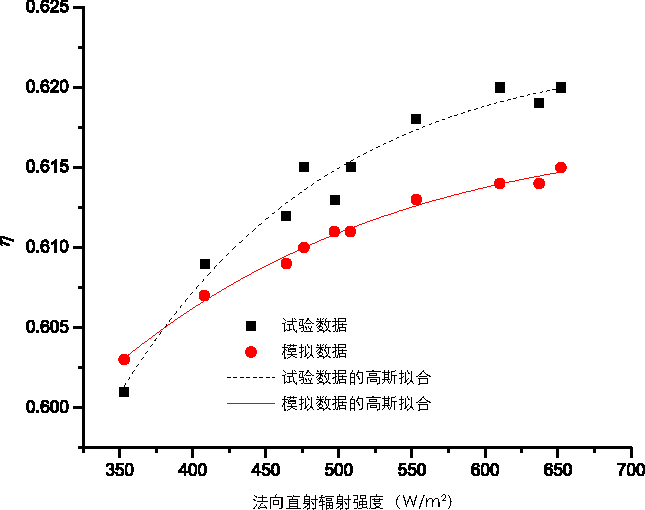
\includegraphics[width=0.7\textwidth]{fig/I_r-eta-trough}
\caption{太阳辐射强度对槽式集热器效率的影响}
\label{fig:I_r-eta-trough}
\end{figure}

可以发现,试验数据和模拟结果具有相同的变化趋势,即槽式集热器的集热效率随着太阳辐射强度的增加而升高。
模拟结果与试验数据的误差很小(小于1\%),但随着太阳辐射强度的增加,误差会有所增大。

\subsubsection{$\dot{m}$的影响}

\begin{table}[htbp]\footnotesize
	\caption{槽式集热器在工况11到工况15条件下的试验结果}
	\begin{center}
	\begin{tabular}{cccccc}
		\toprule
		工况	& DNI ($\mathrm{W/m^2}$)	&	$\dot{m}$ ($\mathrm{kg/s}$)			&	$T_i$ ($\mathrm{K}$)	&	$T_o$ ($\mathrm{K}$)		&	$T_{amb}$ ($\mathrm{K}$)\\
		\midrule
		11	&	612	&	0.1	&	433.2	&	501.0	&	286.3\\
		12	&	615	&	0.2	&	433.2	&	468.2	&	286.4\\
		13	&	615	&	0.3	&	433.2	&	456.7	&	286.6	\\
		14	&	614	&	0.4	&	433.2	&	451.2	&	286.7\\
		15	&	612	&	0.5	&	433.2	&	447.6	&	286.7\\
		\bottomrule
	\end{tabular}
	\end{center}
	\label{tab:ResultOfTrough2}
\end{table}
工况11到工况15的试验结果如表\ref{tab:ResultOfTrough2}所示。这些数据点都是在半个小时内完成采集,以减小太阳辐射变化带来的影响。导热油质量流量对集热器集热效率的影响曲线见图\ref{fig:q_m-eta-trough}。

\begin{figure}[!ht]
\centering
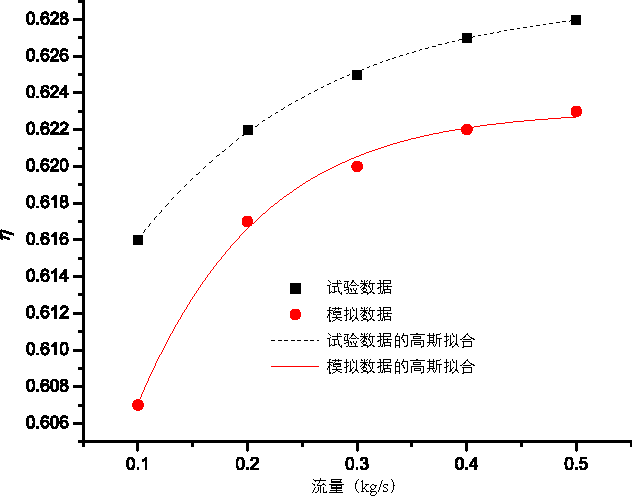
\includegraphics[width=0.7\textwidth]{fig/q_m-eta-trough}
\caption{导热油流量对槽式集热器效率的影响}
\label{fig:q_m-eta-trough}
\end{figure}

可以发现,试验数据和模拟结果具有相同的变化趋势,即槽式集热器的集热效率随着传热流体流量的增加而升高。这是因为,更大的流量将从吸热器带走更多的热量,导致更低的吸热器温度分布,进而使散热损失减小。模拟结果与试验数据存在较小的偏差(误差在0.4\%到0.9\%之间),模拟结果所得的集热效率要低于相应的试验数据得到的集热效率。这是由于模拟过程所采用的整体传热系数公式(见式\ref{eq:U_T_abs})适用于LS-3型的接收器,而对本试验所采用的集热器并不是很适合。未来更多的试验数据可以用来修正此公式,使其更加适用于本试验平台的SEIDO6型接收器。

\subsubsection{$T_i$的影响}

\begin{table}[htbp]\footnotesize
	\caption{槽式集热器在工况16到工况20条件下的试验结果}
	\begin{center}
	\begin{tabular}{cccccc}
		\toprule
		工况	& DNI ($\mathrm{W/m^2}$)	&	$\dot{m}$ ($\mathrm{kg/s}$)			&	$T_i$ ($\mathrm{K}$)	&	$T_o$ ($\mathrm{K}$)		&	$T_{amb}$ ($\mathrm{K}$)\\
		\midrule
		16	&	616	&	0.2	&	413.2	&	449.7	&	289.5\\
		17	&	614	&	0.2	&	423.2	&	458.8	&	288.3\\
		18	&	610	&	0.2	&	433.2	&	467.9	&	288.7	\\
		19	&	618	&	0.2	&	443.2	&	477.7	&	288.9\\
		20	&	615	&	0.2	&	453.2	&	486.8	&	286.3\\
		\bottomrule
	\end{tabular}
	\end{center}
	\label{tab:ResultOfTrough3}
\end{table}
工况16到工况20的试验结果如表\ref{tab:ResultOfTrough3}所示。

Figure~\ref{fig:T_i-eta-trough} shows the influence of inlet temperature on the thermal efficiency of the trough collector.
\begin{figure}[!ht]
\centering
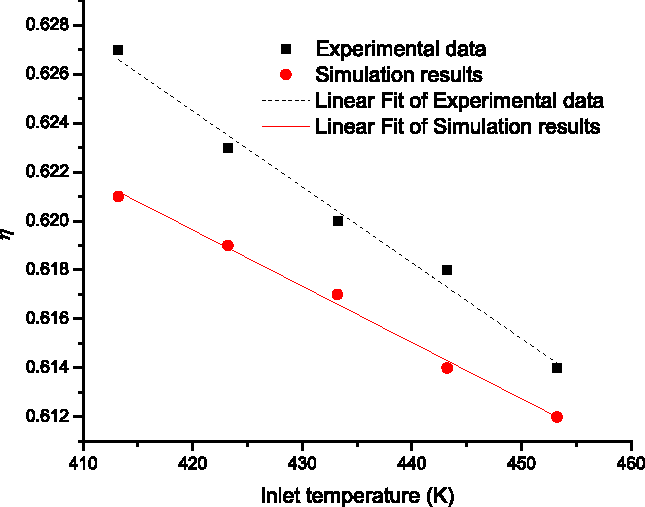
\includegraphics[width=0.7\textwidth]{fig/T_i-eta-trough}
\caption{Influence of inlet temperature on the thermal efficiency}
\label{fig:T_i-eta-trough}
\end{figure}

Both the experimental data and simulation results show that, higher inlet temperature leads to lower efficiency. This is obvious for higher inlet temperature leads to higher receiver temperature distribution and hence more thermal losses. Small deviations also exist between the experimental data and simulation results, between 0.7\% to 1.5\%. The simulation efficiency is lower than corresponding experimental efficiency. This can be interpreted as the same reason of inaccurate thermal loss coefficient $U$.

\subsection{Dish collector experiment result analysis}
Influences of solar irradiance, flow rate and inlet temperature of the working fluid on the collector thermal performance are concerned.
\subsubsection{Influence of $I_r$}

\begin{table}[htbp]\footnotesize
	\caption{Experiment results of 工况 1 to 工况 10 of the dish collector}
	\begin{center}
	\begin{tabular}{cccccc}
		\toprule
		工况	& DNI ($\mathrm{W/m^2}$)	&	$\dot{m}$ ($\mathrm{kg/s}$)			&	$T_i$ ($\mathrm{K}$)	&	$T_o$ ($\mathrm{K}$)		&	$T_{amb}$ ($\mathrm{K}$)\\
		\midrule
		1	&	303	&	0.03	&	423.2	&	552.1	&	282.1\\
		2	&	358	&	0.03	&	423.2	&	576.4	&	282.5\\
		3	&	414	&	0.03	&	423.2	&	602.3	&	283.2	\\
		4	&	426	&	0.03	&	423.2	&	607.5	&	283.4\\
		5	&	512	&	0.03	&	423.2	&	646.0	&	285.0\\
		6	&	596	&	0.03	&	423.2	&	682.7	&	287.4\\
		7	&	620	&	0.03	&	423.2	&	692.4	&	289.2\\
		8	&	641	&	0.03	&	423.2	&	701.5	&	289.5\\
		9	&	658	&	0.03	&	423.2	&	708.7	&	289.4\\
		10	&	683	&	0.03	&	423.2	&	719.4	&	289.5\\
		\bottomrule
	\end{tabular}
	\end{center}
	\label{tab:ResultOfDish1}
\end{table}
Tested results of 工况 1 to 工况 10 are listed in Table~\ref{tab:ResultOfDish1}. It is noteworthy that the measured values of solar irradiance are not evenly distributed due to the uncontrollability and variability of solar radiation intensity.
Figure~\ref{fig:I_r-eta-dish} shows the influence of solar irradiance on the thermal efficiency of the dish collector. Simulation results are also included. The simulation parameters are set to be the same as the experiment. 
%The optical efficiency fo the dish collector is manually reduced to simulate the real situation of the spilled focused spot.
\begin{figure}[!ht]
\centering
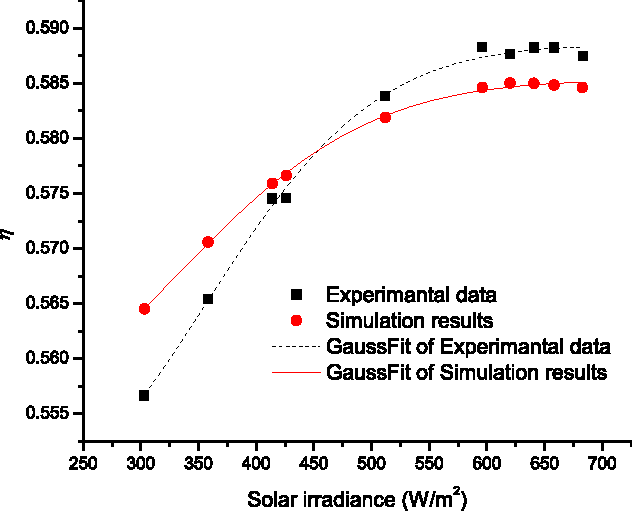
\includegraphics[width=0.7\textwidth]{fig/I_r-eta-dish}
\caption{Influence of solar irradiance on the thermal efficiency}
\label{fig:I_r-eta-dish}
\end{figure}

It can be found that the thermal efficiency increases with solar irradiance when DNI is less than 600$\,\mathrm{W/m^2}$. When DNI is larger than 600$\,\mathrm{W/m^2}$, higher irradiance leads to higher wall temperature and hence more radiation loss, which jeopardizes the thermal efficiency when solar irradiance increases. 
The discrepancy of the experimental data and simulation data may be interpreted for the insulation condition. The out wall temperature of the insulation layer is higher than expected, which proves that the isolation condition is not good enough. 

\begin{figure}[!ht]
\centering
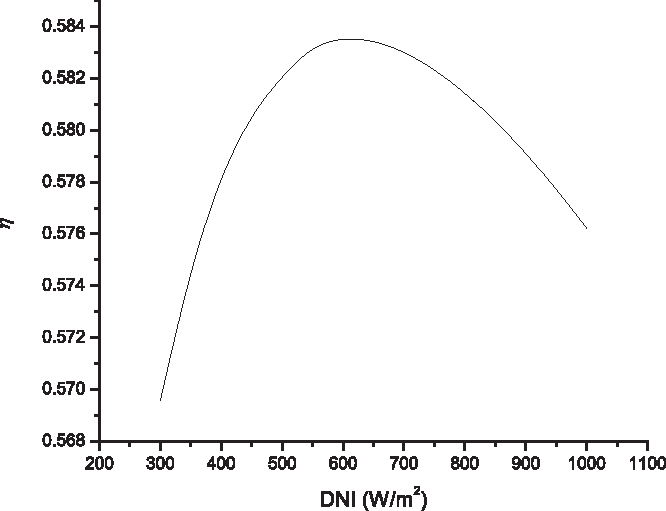
\includegraphics[width=0.7\textwidth]{fig/HigherDNI-eta-dish}
\caption{Simulation results of influence of solar irradiance on the thermal efficiency}
\label{fig:HigherDNI-eta-dish}
\end{figure}
To clearly show the influence of higher DNI, a simulation of the dish collector model was carried out. The inlet air temperature is set to be 423.2$\,\mathrm{K}$, and the flow rate is set to be 0.03$\,\mathrm{kg/s}$. The environment temperature was set to be 283.2$\,\mathrm{K}$ and the wind speed is set to be 0.4$\,\mathrm{m/s}$. The simulation results are shown in Figure~\ref{fig:HigherDNI-eta-dish}. It can be found that there exists an optimum DNI for a specific receiver to achieve the highest thermal efficiency. For the receiver used in the platform, the optimum DNI is about 600$\,\mathrm{W/m^2}$.

%However, it has to be pointed out that these data points were collected in different days, the environment temperature and wind speed may differ. It needs further researches on this topic.

\subsubsection{Influence of $\dot{m}$}

\begin{table}[htbp]\footnotesize
	\caption{Experiment results of 工况 11 to 工况 15 of the dish collector}
	\begin{center}
	\begin{tabular}{cccccc}
		\toprule
		工况	& DNI ($\mathrm{W/m^2}$)	&	$\dot{m}$ ($\mathrm{kg/s}$)			&	$T_i$ ($\mathrm{K}$)	&	$T_o$ ($\mathrm{K}$)		&	$T_{amb}$ ($\mathrm{K}$)\\
		\midrule
		11	&	613	&	0.01	&	423.2	&	950.7	&	286.3\\
		12	&	615	&	0.02	&	423.2	&	783.9	&	286.4\\
		13	&	616	&	0.03	&	423.2	&	691.8	&	286.6	\\
		14	&	614	&	0.04	&	423.2	&	634.9	&	286.7\\
		15	&	613	&	0.05	&	423.2	&	597.8	&	286.7\\
		\bottomrule
	\end{tabular}
	\end{center}
	\label{tab:ResultOfDish2}
\end{table}
Tested results of 工况 11 to 工况 15 are listed in Table~\ref{tab:ResultOfDish2}.
Figure~\ref{fig:q_m-eta-dish} shows the influence of inlet flow rate on the thermal efficiency of the dish collector. The data points on the figure are collected within a short time, so the irradiance can be regarded as unchanged.
\begin{figure}[!ht]
\centering
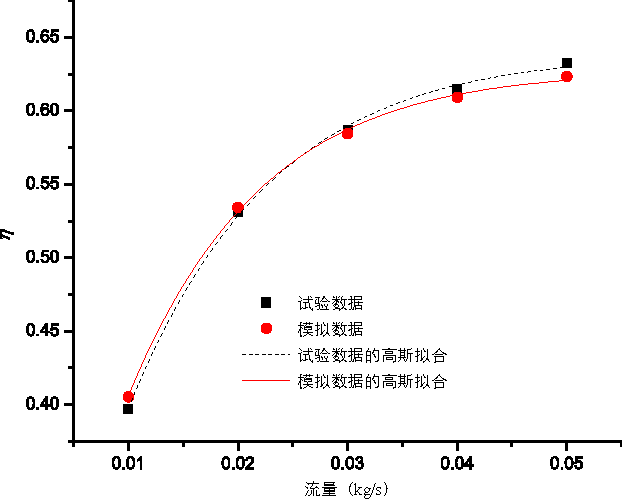
\includegraphics[width=0.7\textwidth]{fig/q_m-eta-dish}
\caption{Influence of inlet flow rate on the thermal efficiency}
\label{fig:q_m-eta-dish}
\end{figure}

It can be found that higher flow rate leads to higher efficiency. This is obvious for higher flow rate takes more heat away from the receiver, leads to lower temperature distribution and hence less thermal losses. The experimental data and simulation result are in good agreement.

\subsubsection{Influence of $T_i$}

\begin{table}[htbp]\footnotesize
	\caption{Experiment results of 工况 16 to 工况 20 of the dish collector}
	\begin{center}
	\begin{tabular}{cccccc}
		\toprule
		工况	& DNI ($\mathrm{W/m^2}$)	&	$\dot{m}$ ($\mathrm{kg/s}$)			&	$T_i$ ($\mathrm{K}$)	&	$T_o$ ($\mathrm{K}$)		&	$T_{amb}$ ($\mathrm{K}$)\\
		\midrule
		16	&	616	&	0.03	&	383.2	&	661.9	&	289.0\\
		17	&	615	&	0.03	&	403.2	&	676.4	&	288.8\\
		18	&	612	&	0.03	&	423.2	&	690.6	&	288.8	\\
		19	&	617	&	0.03	&	443.2	&	707.8	&	288.9\\
		20	&	615	&	0.03	&	463.2	&	722.2	&	288.9\\
		\bottomrule
	\end{tabular}
	\end{center}
	\label{tab:ResultOfDish3}
\end{table}
Tested results of 工况 16 to 工况 20 are listed in Table~\ref{tab:ResultOfDish3}.
Figure~\ref{fig:T_i-eta-dish} shows the influence of inlet flow rate on the thermal efficiency of the dish collector.
\begin{figure}[!ht]
\centering
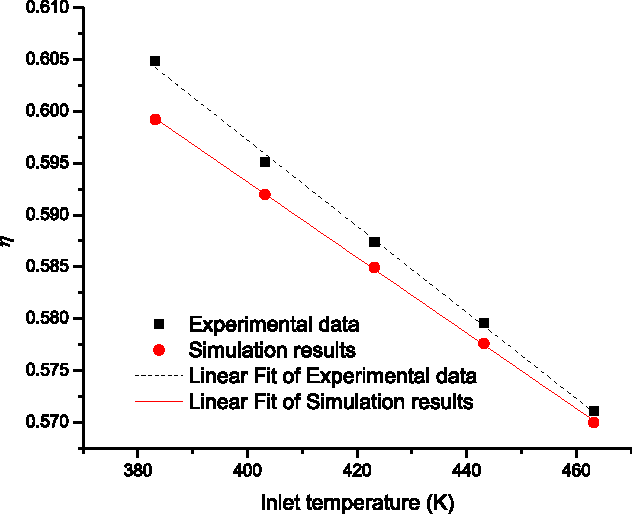
\includegraphics[width=0.7\textwidth]{fig/T_i-eta-dish}
\caption{Influence of inlet temperature on the thermal efficiency}
\label{fig:T_i-eta-dish}
\end{figure}

It can be found that higher inlet temperature leads to lower efficiency, This is obvious for higher inlet temperature leads to higher temperature distribution and hence more thermal losses. The experimental data and simulation result are in good agreement.

\section{Conclusion}

The solar thermal power platform is a good start for the cascade solar thermal system. This chapter introduces the components and the circuits of the platform. According to the features of solar irradiance, special experiment cases are designed to investigate the impact of different factors on the system performance. Experiment steps are carefully arranged.
Tests of the trough collector and the dish collector are carried out and the experimental results are collected for analysis. 

The influence of solar irradiance, flow rate and inlet temperature of the working fluid on the performance of the collector model is investigated. The established trough collector model and dish collector model are validated by the experimental data.

The analysis of experimental data and simulation results shows that

\begin{enumerate}[label=(\arabic*)]
\item The thermal efficiency of trough collectors is between 60.1\% and 62.8\% and the thermal efficiency of dish collectors is between 39.7\% and 63.3\% under the experimental conditions.
\item With regard to the effect of the considered factors on the performance of the collectors, the experimental data and the simulation results have the same trend. Higher working fluid flow rate leads to higher thermal efficiency, while higher working fluid inlet temperature leads to lower thermal efficiency.
\item For a specific dish receiver, there exists an optimum DNI to obtain the highest thermal efficiency.
\item The discrepancy of the experimental data and simulation results of the trough collector indicates that the thermal loss coefficient used in the modeling process is not ideal for the trough product used in the platform. It needs to be revised in the future.
\item The discrepancy of the experimental data and simulation results of the dish collector indicates that the thermal insulation of the dish collector needs to be inspected and strengthened.
\end{enumerate}